\section{\textbf{Methods:} adaptive RR for addressing the high RR dilemma}
\vskip -0.5em
Drawing upon the refined understanding of plasticity loss, this section introduces \textit{Adaptive RR} to tackle the high RR dilemma in VRL.
Extensive evaluations demonstrate that \textit{Adaptive RR} strikes a superior trade-off between reuse frequency and plasticity loss, thereby improving sample efficiency.

\textbf{High RR Dilemma.}~~
Increasing the replay ratio (RR), which denotes the number of updates per environment interaction, is an intuitive strategy to further harness the strengths of off-policy algorithms to improve sample efficiency.
However, recent studies~\citep{breaking_RR_barrier, Regulating_Overfitting} and the results in Figure~\ref{fig:high RR} consistently reveal that adopting a higher static RR impairs training efficiency.


% The replay ratio(RR), defined as the number of gradient updates performed per environment step, is fundamental to training off-policy RL agents.
% We explore the impact of various RR values on sample efficiency in DMC tasks, as depicted in Figure~\ref{fig:high RR}. The results align with the high RR dilemma.

\begin{figure}[hb]
  \centering
  \vspace{-1\baselineskip}
  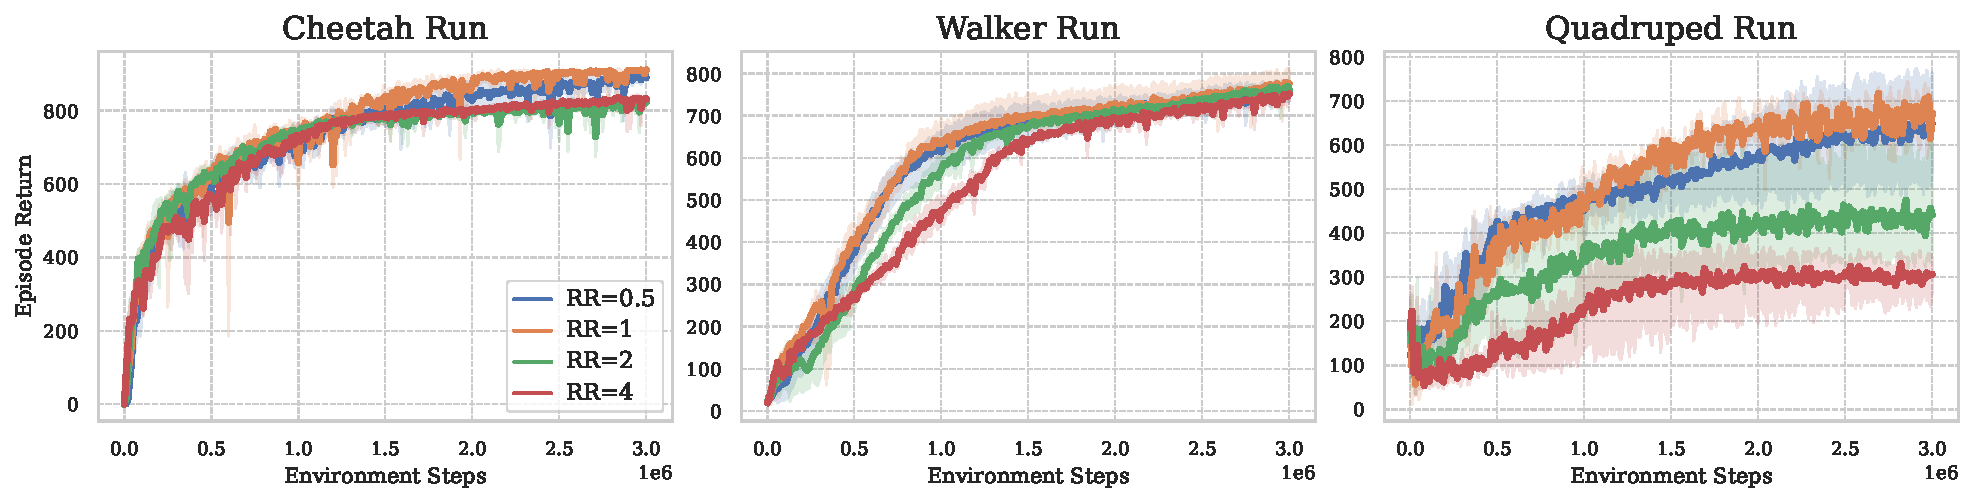
\includegraphics[width=\textwidth]{Figures/4Solutions/High_RR.pdf} 
  \vspace{-2\baselineskip}
    \caption{Training curves across varying RR values. Despite its intent to enhance sample efficiency through more frequent updates, an increasing RR value actually undermines training.}
    \label{fig:high RR}
  % \vspace{-0.5\baselineskip}
\end{figure}

\vspace{-0.5\baselineskip}
\begin{wrapfigure}[14]{r}{0.4\textwidth}
  \vspace{-1.5\baselineskip}  
  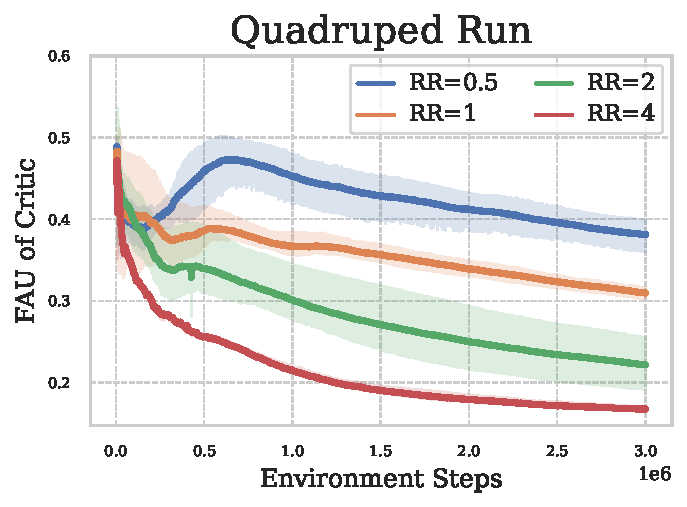
\includegraphics[width=0.4\textwidth]{Figures/4Solutions/FAU_High_RR_QR.pdf}
  \vspace{-1.5\baselineskip}
  \caption{The FAU of critic across varying RR values. A larger RR value leads to more severe plasticity loss.}
  \label{fig:FAU_High_RR}
\end{wrapfigure}
The fundamental mechanism behind this counterintuitive failure of high RR is widely recognized as the intensified plasticity loss~\citep{primacy_bias,dormant_neuron}.
As illustrated in Figure~\ref{fig:FAU_High_RR}, increasing RR results in a progressively exacerbated plasticity loss during the early stages of training.
Increasing RR from $0.5$ to $1$ notably diminishes early-stage plasticity, but the heightened reuse frequency compensates, resulting in a marginal boost in sample efficiency.
However, as RR continues to rise, the detrimental effects of plasticity loss become predominant, leading to a consistent decline in sample efficiency.
When RR increases to $4$, even with the intervention of DA, there's no discernible recovery of the critic's plasticity in the early stages, culminating in a catastrophic loss.
An evident high RR dilemma quandary arises: while higher reuse frequency holds potential for improving sample efficiency, the exacerbated plasticity loss hinders this improvement.

% \ls{relationship between plasticity loss and RR dilemma.}
% \ls{it is still not clear how and why the proposed method can solve this dilemma. We should put more effort into giving a deep interpretation of the proposed methods. Experiments are the results rather than the core reason it works.}
% \ls{We may borrow some insight from curriculum learning on the progressive increasing ratio.}

\textbf{Can we adapt RR instead of setting a static value?}~~
Previous studies addressing the high RR dilemma typically implement interventions to mitigate plasticity loss while maintaining a consistently high RR value throughout training~\citep{breaking_RR_barrier, dormant_neuron, Plasticity_Injection}.
Drawing inspiration from the insights in Section~\ref{Sec: Stages}, which highlight the varying plasticity loss characteristics across different training stages, an orthogonal approach emerges: \textbf{\textit{why not dynamically adjust the RR value based on the current stage?}}
Initially, a low RR is adopted to prevent catastrophic plasticity loss.
In later training stages, RR can be raised to boost reuse frequency, as the plasticity dynamics become benign.
This balance allows us to sidestep early high RR drawbacks and later harness the enhanced sample efficiency from greater reuse frequency.
Furthermore, the observations in Section~\ref{Sec: Modules} have confirmed that the critic's plasticity, as measured by its FAU, is the primary factor influencing sample efficiency.
This implies that the FAU of critic module can be employed adaptively to identify the current training stage.
Once the critic's FAU has recovered to a satisfactory level, it indicates the agent has moved beyond the early training phase prone to catastrophic plasticity loss, allowing for an increase in the RR value. 
Based on these findings and considerations, we propose our method, \textit{Adaptive RR}.

% \vspace{-0.5\baselineskip}
\begin{tcolorbox}[enhanced,colback=white,%
    colframe=C1!75!black, attach boxed title to top right={yshift=-\tcboxedtitleheight/2, xshift=-.75cm}, title=\textbf{Adaptive Replay Ratio}, coltitle=C1!75!black, boxed title style={size=small,colback=white,opacityback=1, opacityframe=0}, size=title, enlarge top initially by=-\tcboxedtitleheight/2]
    \vspace{0.3em}
\textcolor{C1!25!black}{\textit{Adaptive RR} adjusts the ratio according to the current plasticity level of critic, utilizing a low RR in the early stage and transitioning it to a high value after the plasticity recovery stages.}
\vspace{0.2em}
\end{tcolorbox}



% To be precise, in order to mitigate irreversible plasticity loss that could notably compromise sample efficiency, we adopt a low RR in the early training stage. 
% As the training progresses, we monitor the critic network's FAU at specified intervals. 
% When the difference in FAU between consecutive checkpoints falls below a predetermined threshold, indicating the conclusion of the early stage, we adjust the RR upward to enhance sample efficiency.
% Despite its simplicity, our Adaptive RR can be integrated into various off-policy RL training methods.
%Furthermore, A-RR can naturally be applied to a wide range of base RL training methods.

% \begin{minipage}{.5\linewidth}
% \begin{algorithm}[H]
%  \caption{Adaptive RR}
%   \begin{algorithmic}[1]
%     \Require Check interval $K$, threshold $\tau$, total steps $T$
%     \State Initialize RL training with a low RR
%      \While{$t < T$} 
%      %\Comment{Where $T$ is the total number of steps}
%         \If{$t\%K=0$ and $|\Phi_{C}^{t} - \Phi_{C}^{t-K}|<\tau$}
%             \State Switch to high RR 
%         \EndIf
%         \State Continue RL training with the current RR
%         \State Increment step $t$
%      \EndWhile
%   \end{algorithmic}
%   \label{algo:main}
% \end{algorithm}
% \end{minipage}

% \vspace{-0.2\baselineskip}
\textbf{Evaluation on DeepMind Control Suite.}~~
We then evaluate the effectiveness of \textcolor{AARed}{\textit{Adaptive RR}}\githubfootnote{Our code is available at: \url{https://github.com/Guozheng-Ma/Adaptive-Replay-Ratio}} in improving the sample efficiency of VRL algorithms.
Our experiments are conducted on six challenging continuous DMC tasks, which are widely perceived to significantly suffer from plasticity loss~\citep{Enhancing_Generalization_Plasticity}.
We select two static RR values as baselines:
\textcolor{AAGray}{$\bullet$ Low RR=$0.5$}, which exhibits no severe plasticity loss but has room for improvement in its reuse frequency.
\textcolor{AABlue}{$\bullet$ High RR=$2$}, which shows evident plasticity loss, thereby damaging sample efficiency.
Our method, \textcolor{AARed}{\textit{Adaptive RR}}, starts with RR=$0.5$ during the initial phase of training, aligning with the default setting of DrQ-v2. Subsequently, we monitor the FAU of the critic module every $50$ episodes, \textit{i.e.}, $5 \times 10^4$ environment steps.
When the FAU difference between consecutive checkpoints drops below a minimal threshold (set at $0.001$ in our experiments), marking the end of the early stage, we adjust the RR to $2$.
Figure~\ref{fig:arr_main_result} illustrates the comparative performances.
\textcolor{AARed}{\textit{Adaptive RR}} consistently demonstrates superior sample efficiency compared to a static RR throughout training.

\begin{figure}[ht]
  \centering
  \vspace{-0.5\baselineskip}
  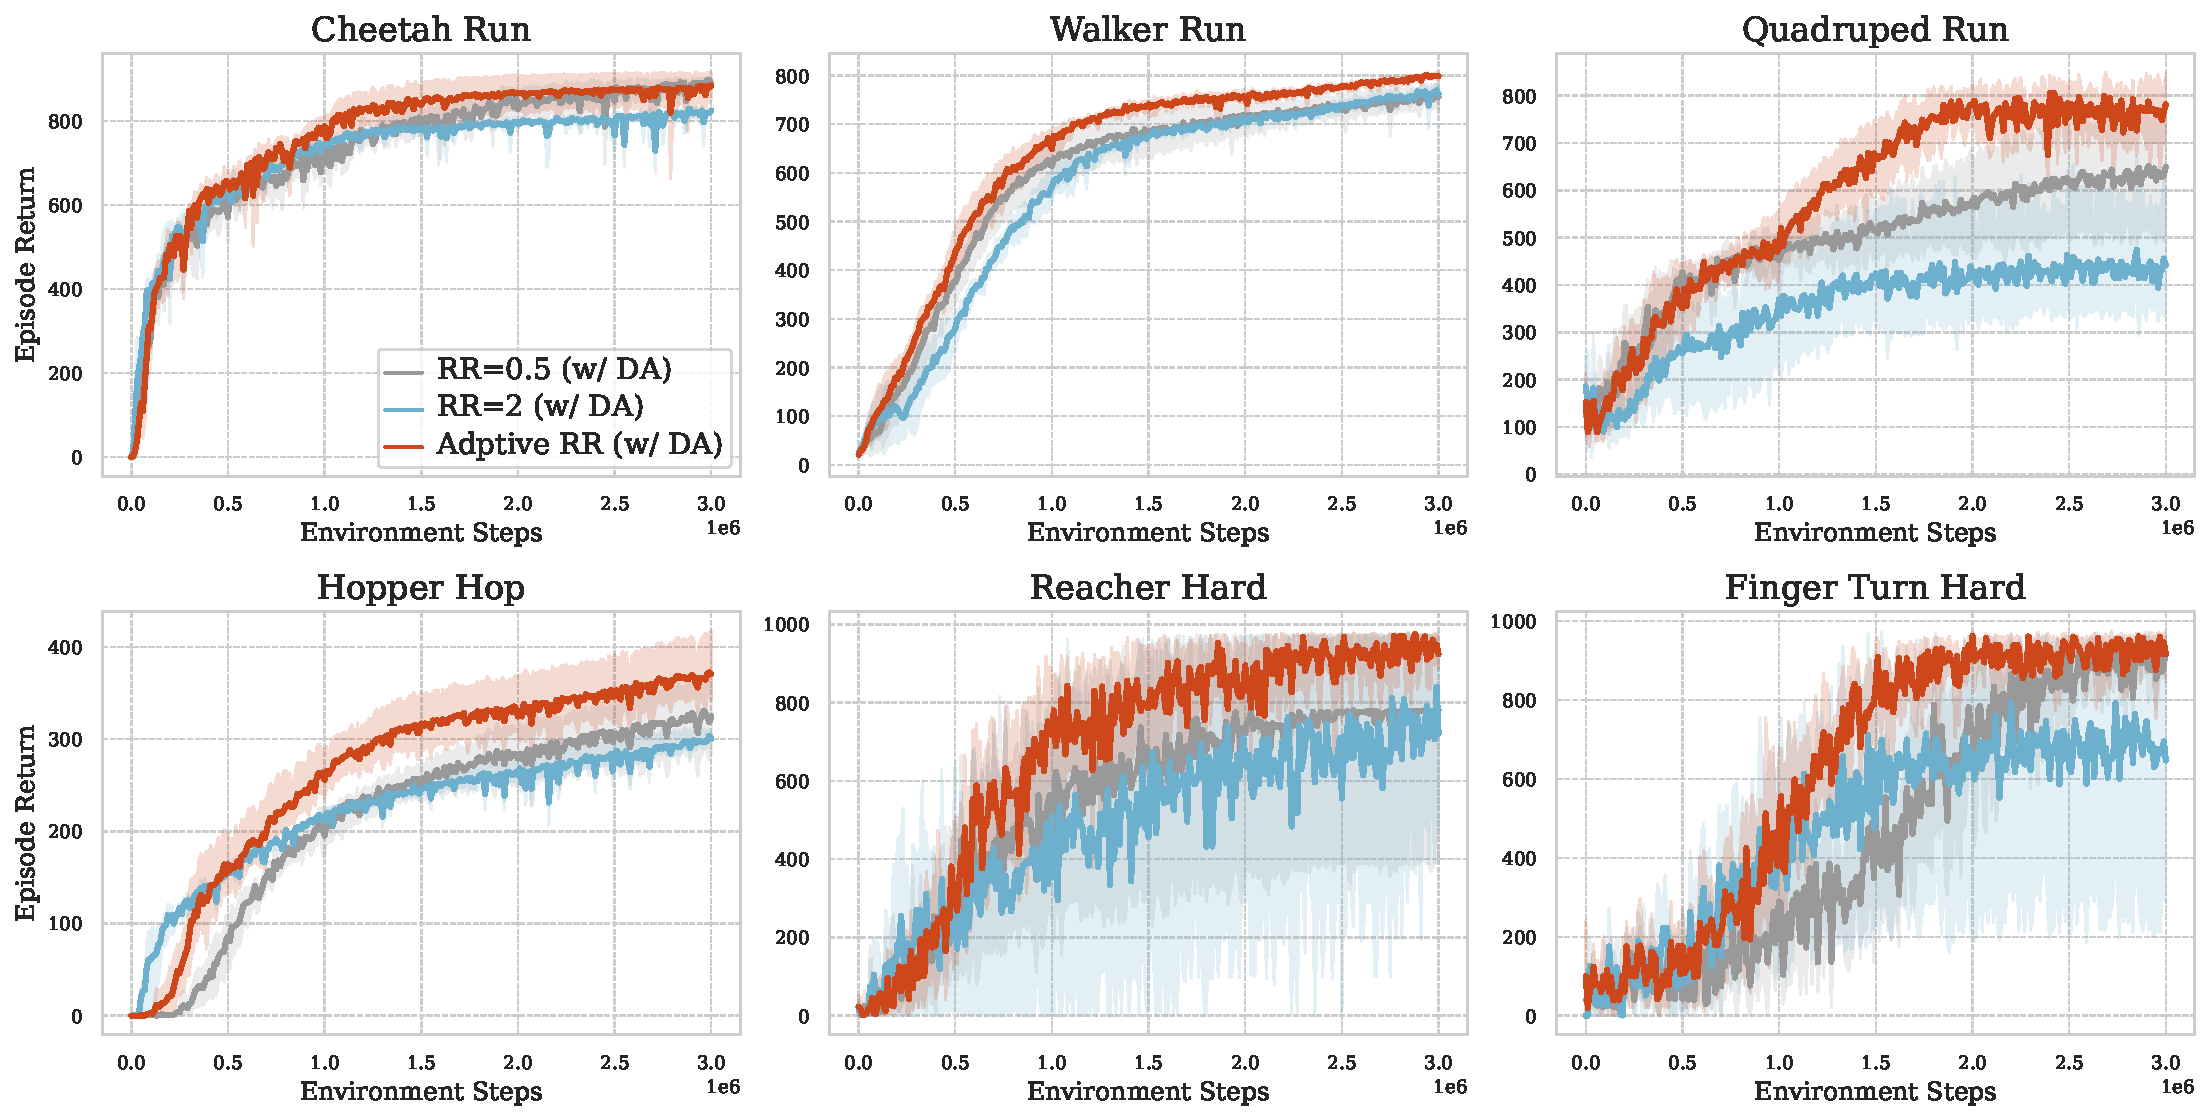
\includegraphics[width=\textwidth]{Figures/4Solutions/ARR_Results.pdf} 
  \vspace{-1.5\baselineskip}
    \caption{Training curves of various RR settings across 6 challenging DMC tasks. \textcolor{AARed}{\textbf{\textit{Adaptive RR}}} demonstrates superior sample efficiency compared to both static \textcolor{AAGray}{low RR} and \textcolor{AABlue}{high RR} value.}
    \label{fig:arr_main_result}
  % \label{DMC Training}
\end{figure}
\vspace{-\baselineskip}
\begin{figure}[ht]
  \centering
  \vspace{-0.5\baselineskip}
  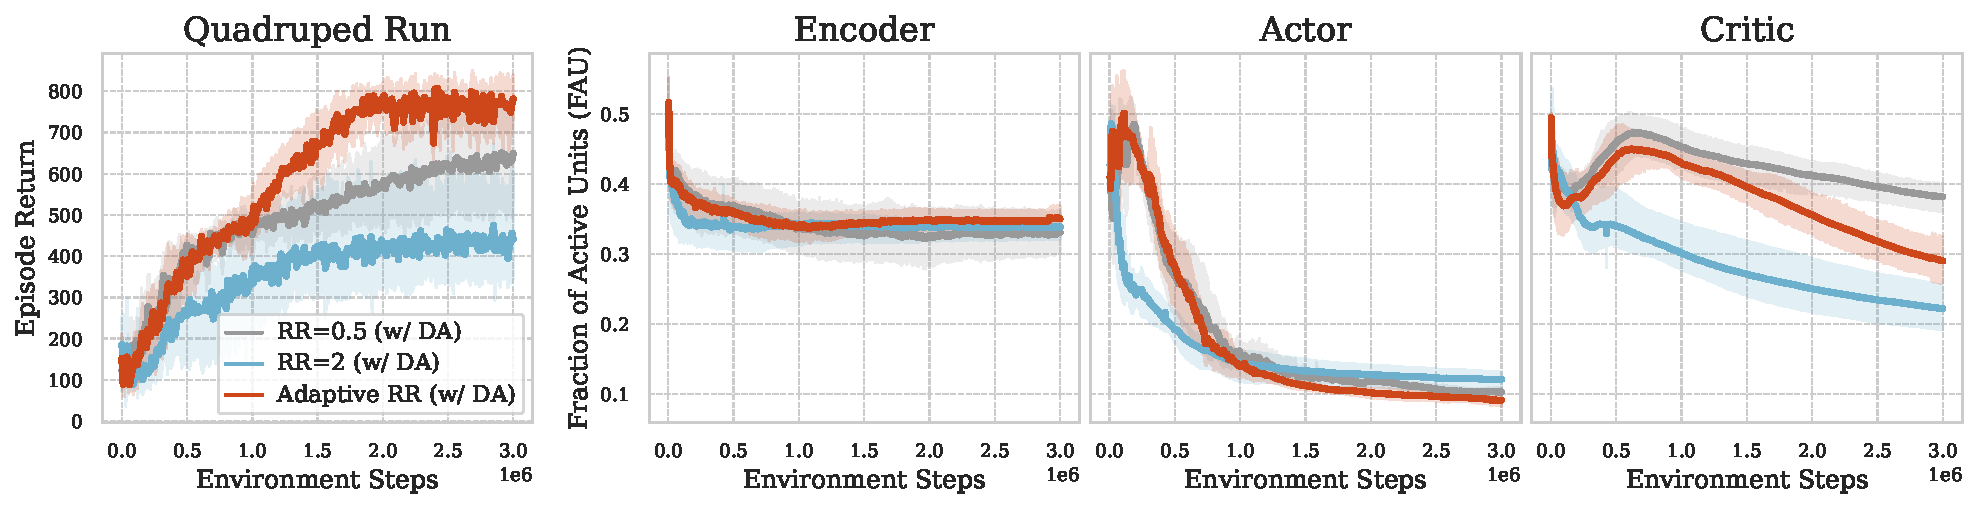
\includegraphics[width=\textwidth]{Figures/4Solutions/FAU_ARR_QR.pdf}
  \vspace{-1.5\baselineskip}
  \caption{Evolution of FAU across the three modules in the Quadruped Run task under different RR configurations.
  The critic's plasticity is most influenced by different RR settings. Under \textcolor{AABlue}{high RR}, the critic's plasticity struggles to recover in early training.
  In contrast, \textcolor{AARed}{\textit{Adaptive RR}} successfully mitigates catastrophic plasticity loss in the early phases, yielding the optimal sample efficiency.}
  \label{figure:ARR_FAU}
\end{figure}

\vspace{-0.7\baselineskip}
Through a case study on Quadruped Run, we delve into the underlying mechanism of \textcolor{AARed}{\textit{Adaptive RR}}, as illustrated in Figure~\ref{figure:ARR_FAU}. 
Due to the initial RR set at $0.5$, the critic's plasticity recovers promptly to a considerable level in the early stages of training, preventing catastrophic plasticity loss as seen with RR=$2$.
After the recovery phases, \textcolor{AARed}{\textit{Adaptive RR}} detects a slow change in the critic's FAU, indicating it's nearing a peak, then switch the RR to a higher value.
Within our experiments, the switch times for the five seeds occurred at: $0.9$M, $1.2$M, $1.1$M, $0.95$M, and $0.55$M.
After switching to RR=$2$, the increased update frequency results in higher sample efficiency and faster convergence rates.
Even though the critic's FAU experiences a more rapid decline at this stage, this benign loss doesn't damage training.
Hence, \textcolor{AARed}{\textit{Adaptive RR}} can effectively exploits the sample efficiency advantages of a high RR, while adeptly avoiding the severe consequences of increased plasticity loss.
% Furthermore, \textcolor{AARed}{\textit{Adaptive RR}} is orthogonal to other interventions aimed at preserving plasticity. Consequently, they can be integrated seamlessly to amplify the VRL's sample efficiency.

\begin{table}[ht]
\centering
\vspace{-0.5\baselineskip}
\caption{Comparison of Adaptive RR versus static RR with Reset and ReDo implementations. The average episode returns are averaged over 5 seeds after training for 2M environment steps.}
\vspace{-0.5\baselineskip}
\renewcommand{\arraystretch}{1.15}
\setlength{\tabcolsep}{7pt}
\resizebox{\columnwidth}{!}{
\begin{tabular}{lccccccc}
\toprule
Average Episode Return& \multicolumn{3}{c}{RR=0.5}   & \multicolumn{3}{c}{RR=2} & \multicolumn{1}{c}{Adaptive RR} \\ 
\cmidrule(lr){2-4} \cmidrule(lr){5-7} \cmidrule(lr){8-8} 
% 2M Env Steps & RR=0.5 & RR=0.5 & RR=0.5 & RR=2 & RR=2 & RR=2 & Adaptive RR \\
(After 2M Env Steps) & \footnotesize{\tt default} & \footnotesize{\tt Reset}& \footnotesize{\tt ReDo} & \footnotesize{\tt default} & \footnotesize{\tt Reset} & \footnotesize{\tt ReDo} & \footnotesize{\tt{RR:0.5to2}} \\
\midrule
Cheetah Run & $828 \pm 59\hphantom{0}$ & $799 \pm 26\hphantom{0}$ & $788 \pm 5\hphantom{00}$ & $793 \pm 9\hphantom{00}$ & $\bestscore{885 \pm 20}$ & $873 \pm 19$ & $880 \pm 45$ \\
Walker Run & $710 \pm 39\hphantom{0}$ & $648 \pm 107$ & $618 \pm 50\hphantom{0}$ & $709 \pm 7\hphantom{00}$ & $749 \pm 10$ & $734 \pm 16$ &  $\bestscore{758 \pm 12}$ \\
Quadruped Run & $579 \pm 120$ & $593 \pm 129$ & $371 \pm 158$ & $417 \pm 110$ & $511 \pm 47$ & $608 \pm 53$ & $\bestscore{784 \pm 53}$ \\
\bottomrule
\end{tabular}
}
\label{table:redo}
\end{table}

\vspace{-0.5\baselineskip}
We further compare the performance of Adaptive RR with that of employing Reset~\citep{primacy_bias} and ReDo~\citep{dormant_neuron} under static RR conditions.
Although Reset and ReDo both effectively mitigate plasticity loss in high RR scenarios, our method significantly outperforms these two approaches, as demonstrated in Table~\ref{table:redo}
This not only showcases that Adaptive RR can secure a superior balance between reuse frequency and plasticity loss but also illuminates the promise of dynamically modulating RR in accordance with the critic's overall plasticity level as an effective strategy, alongside neuron-level network parameter resetting, to mitigate plasticity loss.

\begin{wrapfigure}[10]{r}{0.5\textwidth}
\centering
\vspace{-\baselineskip}
\captionof{table}{Summary of Atari-100K results. Comprehensive scores are available in Appendix~\ref{Evaluation on Atari}.}
\vspace{-0.5\baselineskip}
\renewcommand{\arraystretch}{1.15}
\setlength{\tabcolsep}{2pt}
\resizebox{0.5\columnwidth}{!}{
\begin{tabular}{lccccc}
\toprule
\multirow{2}*{\textit{Metrics}} & \multicolumn{3}{c}{DrQ($\epsilon$)}  & {ReDo}& {Adaptive RR}\\
\cmidrule(lr){2-4} \cmidrule(lr){5-5} \cmidrule(lr){6-6} 
& \footnotesize{\tt{RR=0.5}} & \footnotesize{\tt{RR=1}} & \footnotesize{\tt{RR=2}}  & \footnotesize{\tt{RR=1}}&
\footnotesize{\tt{RR:0.5to2}}\\
\midrule
\textit{Mean HNS ($ \% $)} & $42.3$ & $41.3$ & $35.1$& $42.3$ & $\bestscore{55.8}$\\
\textit{Median HNS ($ \% $)} &$22.6$ & $30.3$ & $26.0$ & $41.6$ & $\bestscore{48.7}$ \\
\textit{$\#$ Superhuman} &$3$ & $1$ & $1$ & $2$ &$\bestscore{4}$\\
\textit{$\#$ Best} & $0$ & $2$ & $1$ & $3$ & $\bestscore{11}$ \\
\bottomrule
\end{tabular}
\label{table:atari-short}
}
\end{wrapfigure}
\textbf{Evaluation on Atari-100k.}~
To demonstrate the applicability of Adaptive RR in discrete-action tasks we move our evaluation to the Atari-100K benchmark~\citep{kaiser2019model}, assessing Adaptive RR against three distinct static RR strategies across 17 games.
In static RR settings, as shown in Table~\ref{table:atari-short}, algorithm performance significantly declines when RR increases to 2, indicating that the negative impact of plasticity loss gradually become dominant.
However, Adaptive RR, by appropriately increasing RR from 0.5 to 2 at the right moment, can effectively avoid catastrophic plasticity loss, thus outperforming other configurations in most tasks.